\documentclass[12pt]{article}

\usepackage{fontawesome}
\usepackage{hyperref}
\usepackage{xurl}
\usepackage{graphicx}


\hypersetup{
    colorlinks=false,
    pdfborder={0 0 0},
}


\title{Introduction to Databases}
\author{
        Adrianna Holden-Gouveia \\
        Website: \url{https://aholdengouveia.name}\\ 
        \date{\vspace{-5ex}}
        %Email: \href{mailto:admin@aholdengouveia.name}{admin@aholdengouveia.name} \\
        \faLinkedin{: aholdengouveia} \\
        \faGithub {: aholdengouveia} \\
        %\faTwitter {: aholdengouveia} \\
        }

%S\date{\today}


\begin{document}    

\maketitle

%\begin{abstract}
%This is a template for Linux Administration Lab work
%\end{abstract}
%\tableofcontents

\section*{Objectives:}
\begin{itemize}
    \item The objective of this lab assignment is to help students gain a basic understanding of the differences between spreadsheets and databases, without requiring prior knowledge of specific software. Through hands-on exploration, students will compare the features and potential use cases of these tools.
\end{itemize}


References, a video, a PowerPoint and some notes are available at my website
\url {https://www.aholdengouveia.name/IntroData/introdatabases.html}

For this lab you'll be using LibreOffice Base.  The documentation can be found at \url{https://books.libreoffice.org/en/BG73/BG7301-IntroductionToBase.html#toc26}

You should get your data into a database, you may use a single table or multiple tables. LibreOffice Base is a Database front end using a Graphical User Interface (GUI), there are a lot of other ways you can get your data into a database as well and interact with it. We will be talking about those soon. After your data is in the database, answer the following questions


%\section*{Complete the following problems}


\subsection*{Moving your data to a Database}
    \begin{enumerate}
        \item How long did it take you to move your data?
        \item Did you create one table or more? Why did you make the choice you did?
        \item Compared to a spreadsheet how difficult would you say it was to move your data into the database?
        \item What are your thoughts on the documentation? Did you have to use other resources? 
        \item Screenshot of your data in the database.  Use your best judgement for how to illustrate that and what screenshot to take.  Why did you pick what you did?
        \begin{figure}[h!]
            \centerline{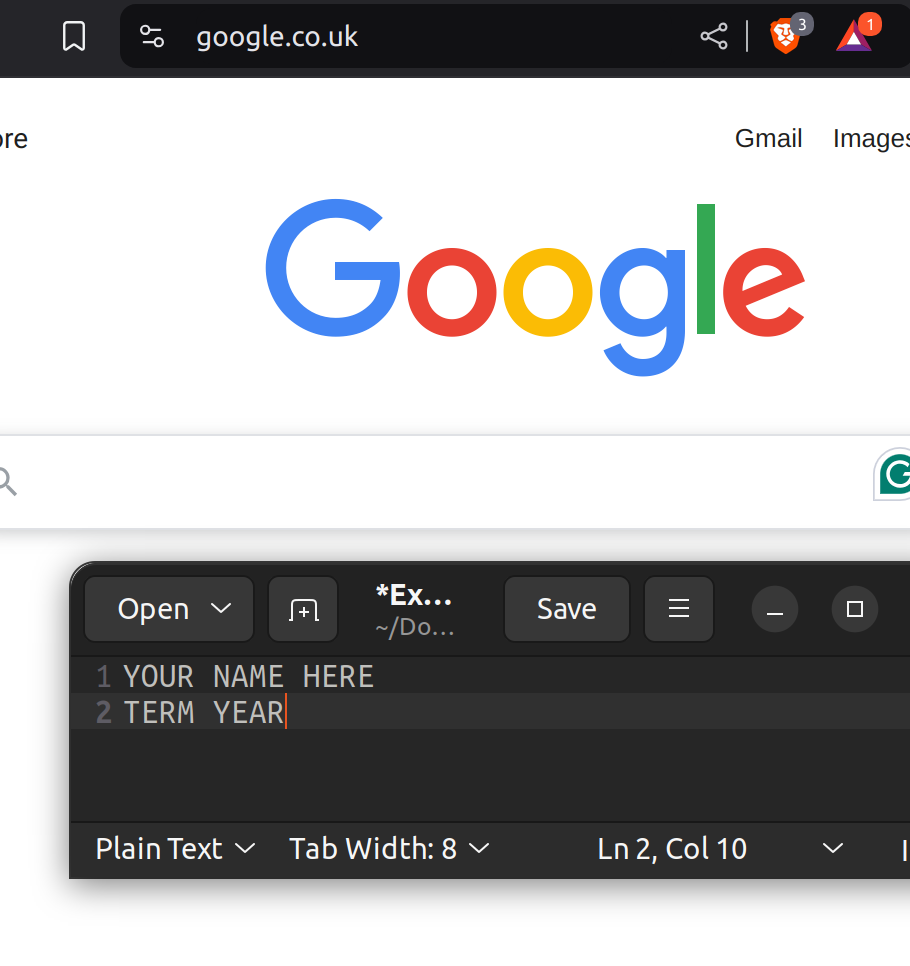
\includegraphics[scale=.2]{ExampleScreenshot.png}}
            \caption{This is an image of what each of your screenshots should look like}

            \end{figure} 
    \end{enumerate}

    \subsection*{Database questions}
    \begin{enumerate}
        \item How does your data look different in the database instead of your original spreadsheet view?
        \item How would you add another record to your database?  Go ahead and add something that fits in with the data you've collected.  How was adding this different then if you added to a spreadsheet?
        \item How would you edit a record? Go ahead and change one of the records in some way, this could be fixing information, adding information, or just changing something. 
        \item If you needed to find a specific record or piece of information in your database, how would you go about doing that? Give one link or reference that you used to help.

    \end{enumerate}

\section*{Deliverables}
\begin{enumerate}
    \item A text document with the answers to the questions given about getting your data into the database you're creating
    \item A text Document with the answers to the questions about the database you've created
    \item All requested screenshots, clearly labeled to show what they are for
    \item Find one reference for how to use LibreOffice Base, this could be an article, or video, or documentation, or activity.  Include the URL here and write a short review of it. Your short review should be more then one paragraph and less then one page.
    \item Your database, make sure you're submitting a database, not spreadsheet. 
\end{enumerate} 
\end{document}